\section{Introduction}

Recognising facial expressions and the underlying emotions is important for human interaction. Through those facial expressions humans can detect and sense the underlying emotional state of their peers, playing a vital part in social discourse. The ability to recognise facial expressions artificially opens up many applications in human-computer interaction, like market research and content evaluation.

A key figure in the study of human emotion and its perception through facial expressions was Paul Ekman \cite{ekman1987universals} \cite{ekman1992basic} \cite{ekman2013emotion}. The focus of his work was to demonstrate that emotions express themselves universally in facial expressions, and are discrete classes of a emotional set \cite{ekman1987universals}.

Going forward several years into the mid-90s, Picard consolidated ideas of computing and measuring affect as a field of computer science in her 1995 essay, coining the term Affective Computing \cite{picard2000affective}. A subfield of affective computing is based around recognising affective states from facial expressions by combining advancements in computational ability with the research of Ekman \cite{ekman1987universals} \cite{friesen1978facial} and Russell \cite{russell1980circumplex}. Much of the progress in this field bases its research around several axiomatic assumptions, one of which being that all facial movements are induced by emotion. This is especially problematic if the analysed subject is speaking, since the act of talking also triggers facial movement and thus introduces noise into the input data. An example of this can be seen in figure \ref{fig:mislabel}. 

In this thesis, we explore ways to make facial expression recognition models more robust against speech. We analyse ability of humans to detect and judge facial expressions on talking subjects. To explore this we organised data collection and annotators using a web tool to label parts of an existing dataset (Section \ref{sec:human}). This suggested that \textit{humans are more accurate in judging emotions when confronted with a video instead of single frames}. Humans also were \textit{consistent in regards to the lexical content of the video}, being equally accurate no matter what was being said.

In section \ref{sec:models} we build on the insights from section \ref{sec:human} in two main ways to increase the robustness of facial expression recognition against speech:

\begin{enumerate}
    \item The addition of a \textbf{temporal dimension}: Speech is inherently temporal. We want to utilise this and leverage the contextual nature of the facial movements that relate to speech through temporal compensation.
    \item The inclusion of a \textbf{lexical compensator}: By including lexical compensators, we want to separate facial movements induced by speech from those that are induced by emotion and thus increase the robustness of our models against speech.
\end{enumerate}

We adopt state-of-the-art recurrent deep neural networks to add a temporal dynamic to our network, estimating the emotion over a given time instead of a frame by frame approach of classic facial expression recognition models. Lexical compensators are introduced as separate models that will produce additional inputs for our facial expression recognition model. We follow two approaches from previous work \cite{bursic2020improving} \cite{salman2020style}, and try to build on those. We end up with three different models:

\begin{itemize}
    \item Temporal facial expression recognition model
    \item Temporal facial expression recognition model including LipNet, a model specifically trained for lipreading, as a lexical compensator \cite{bursic2020improving}
    \item Temporal facial expression recognition model including a self-trained style extractor as a lexical compensator \cite{salman2020style}
\end{itemize}

To further analyse our models, we will validate them on separate datasets. One of those datasets will be in German to analyse the impact of a different language to the one used in the training dataset. Details on how we collected the data and the resulting analysis can be found in section \ref{sec:data}.

We conclude that the \textit{temporal compensation is the main factor in creating facial expression recognition models that are robust against speech}. Our experiments in sections \ref{sec:model_results} and \ref{sec:data_discussion} show an increase in performance with more temporal information. \textit{Models with lexical compensation show promise}, but do not significantly outperform models without it in its present state.

\begin{figure}
    \centering
    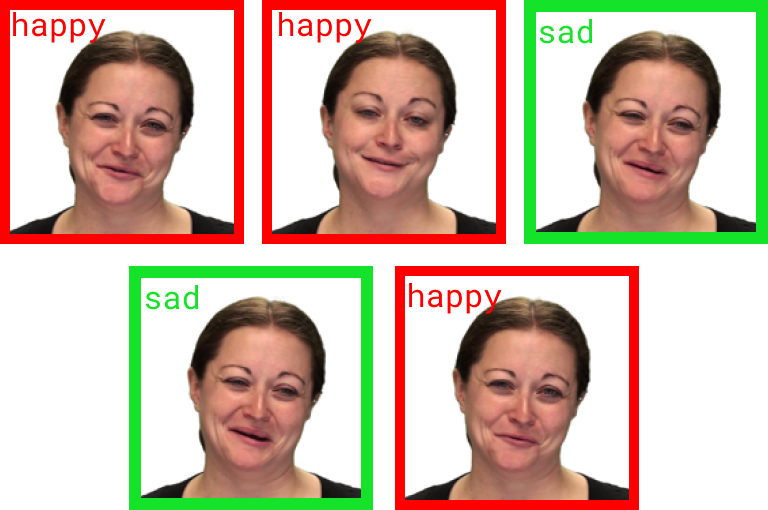
\includegraphics[width=0.8\textwidth]{res/png_backup/mislabel.png}
    \caption{An example of a model automatically predicting emotions from the face of a speaking subject while expressing a \texttt{sad} emotion \cite{livingstone2018ryerson}. Ideally, all frames would be correctly categorized as \texttt{sad}. Because of facial movements related to speech, the model only predicts the correct emotion twice. In this thesis we will work on creating models that are robust against predicting emotions from speaking subjects.}
    \label{fig:mislabel}
\end{figure}